% The five acronym images (unnumbered section, included by % The five acronym images (unnumbered section, included by % The five acronym images (unnumbered section, included by % The five acronym images (unnumbered section, included by \input{easter_eggs_figures}).
% Figures produced by code/easter_egg_images.py (matplotlib/numpy/scipy); every plotted quantity is computed
% from its formula. The numerical self-checks (positive and negative controls) are recorded in
% results/textbook_formalisation_2026/easter_eggs_selfcheck.json; a failing check aborts the script.
\section*{The five images}
\addcontentsline{toc}{section}{The five images}

Each of the five short names of Section~\ref{ch5:acronymes} receives an image here. The tier of the theorem
(\tierA{}) refers to the re-exported Lean statement. The curves, colours and displayed values are numerical
computations \tierX{}: they illustrate a special case of the statement, without proving or extending it.

\begin{figure}[htbp]
\centering
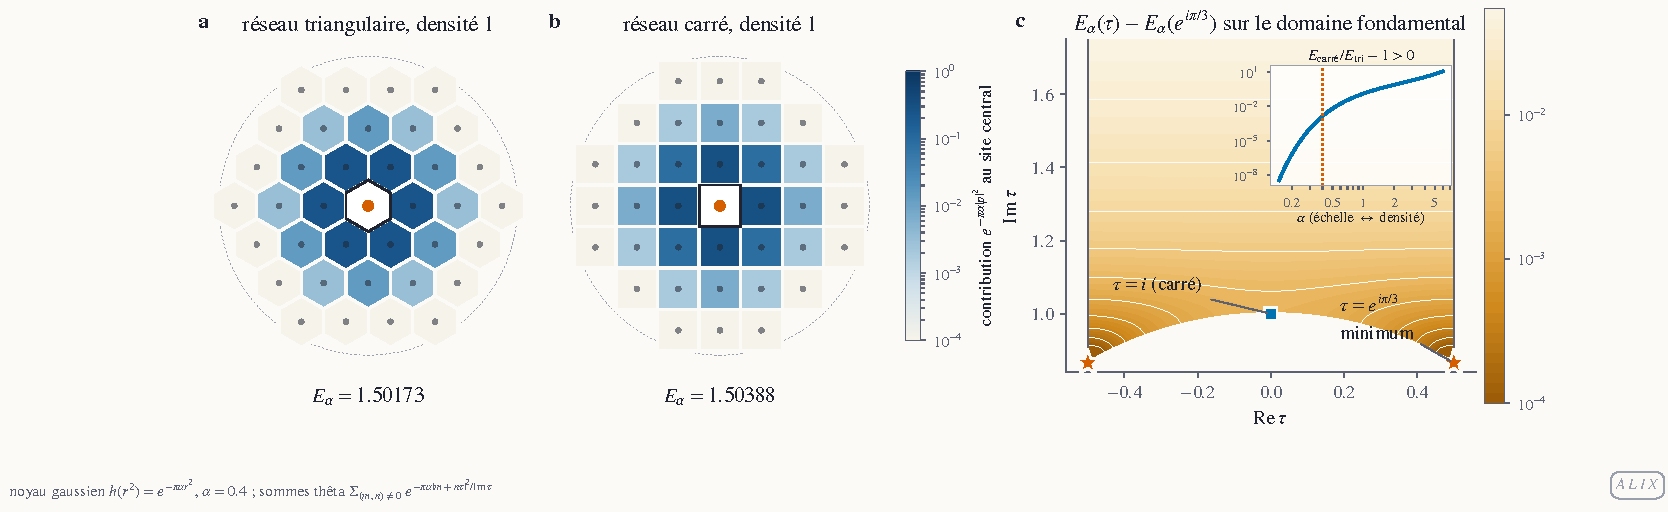
\includegraphics[width=\textwidth]{egg_ALIX.pdf}
\caption{\lean{ALIX}, \emph{A Lattice Is eXtremal}. The theorem \tierA{} (conditional on the upstream theorem
\lean{universal_energy_minimum} of openai/math, AI-generated and not peer reviewed) states that at every density
$\rho>0$ the triangular lattice minimizes the energy of every admissible potential, among all locally finite
configurations of density~$\rho$. The image \tierX{} takes the Gaussian kernel $e^{-\pi\alpha r^2}$, $\alpha=0.4$,
at density~1, and compares \emph{lattices} only. (a)~and~(b): Voronoi cells coloured by the contribution
$e^{-\pi\alpha|p|^2}$ of each site~$p$ to the energy of the central site; $E_\alpha=1.50173$ (triangular)
versus $1.50388$ (square). (c)~The difference $E_\alpha(\tau)-E_\alpha(e^{i\pi/3})$ over the fundamental domain of
lattice shapes, computed by theta sums; the grid minimum (at the equivalent point $-\tfrac12+i\tfrac{\sqrt3}2$, to within one grid step) and five
Nelder--Mead minimizations (to within $10^{-7}$) land back on $\tau=e^{i\pi/3}$. Inset: $E_{\text{square}}/E_{\text{tri}}-1>0$ for
$\alpha\in[0.15, 6]$, that is, for a whole range of densities.}
\label{fig:egg:ALIX}
\end{figure}

\begin{figure}[htbp]
\centering
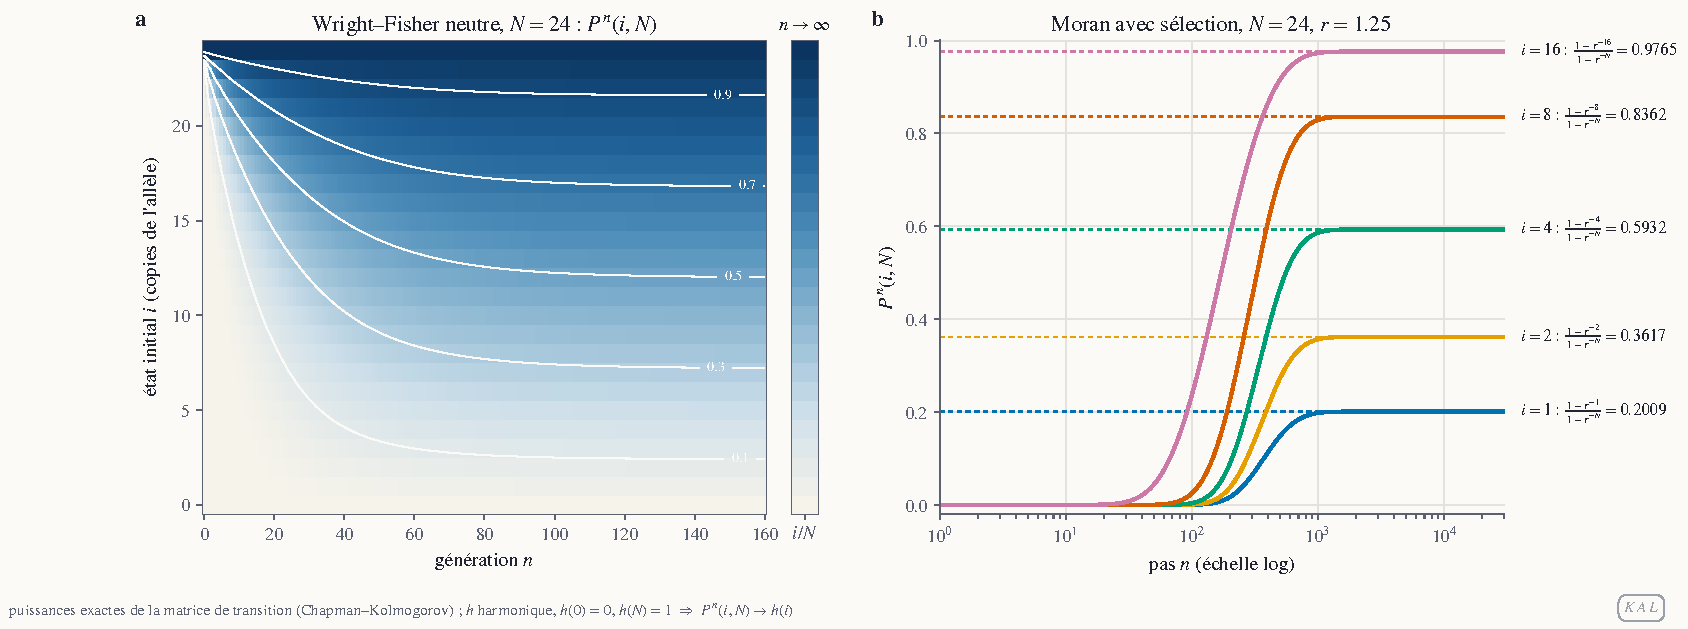
\includegraphics[width=\textwidth]{egg_KAL.pdf}
\caption{\lean{KAL}, \emph{Kolmogorov Absorption Limit}. The theorem \tierA{}: for a chain on
$\{0,\dots,N\}$ with absorbing boundaries, if $h$ is harmonic at the interior states, $h(0)=0$, $h(N)=1$, and the
one-step variance of $h$ is strictly positive, then $P^n(i,N)\to h(i)$ and $P^n(i,0)\to 1-h(i)$. Images
\tierX{}, by exact powers of the transition matrix. (a)~Neutral Wright--Fisher, $N=24$: $P^n(i,N)$
converges to $h(i)=i/N$ (right-hand band); maximal deviation at $n=4096$: $6\cdot10^{-16}$. (b)~Moran with
selection, $N=24$, $r=1.25$: $P^n(i,N)$ tends to $(1-r^{-i})/(1-r^{-N})$ (dotted), deviation
$7\cdot10^{-15}$ at $n=2^{22}$. The harmonicity of both functions $h$ is checked in exact rationals (for Wright--Fisher, at $N=8$).}
\label{fig:egg:KAL}
\end{figure}

\begin{figure}[htbp]
\centering
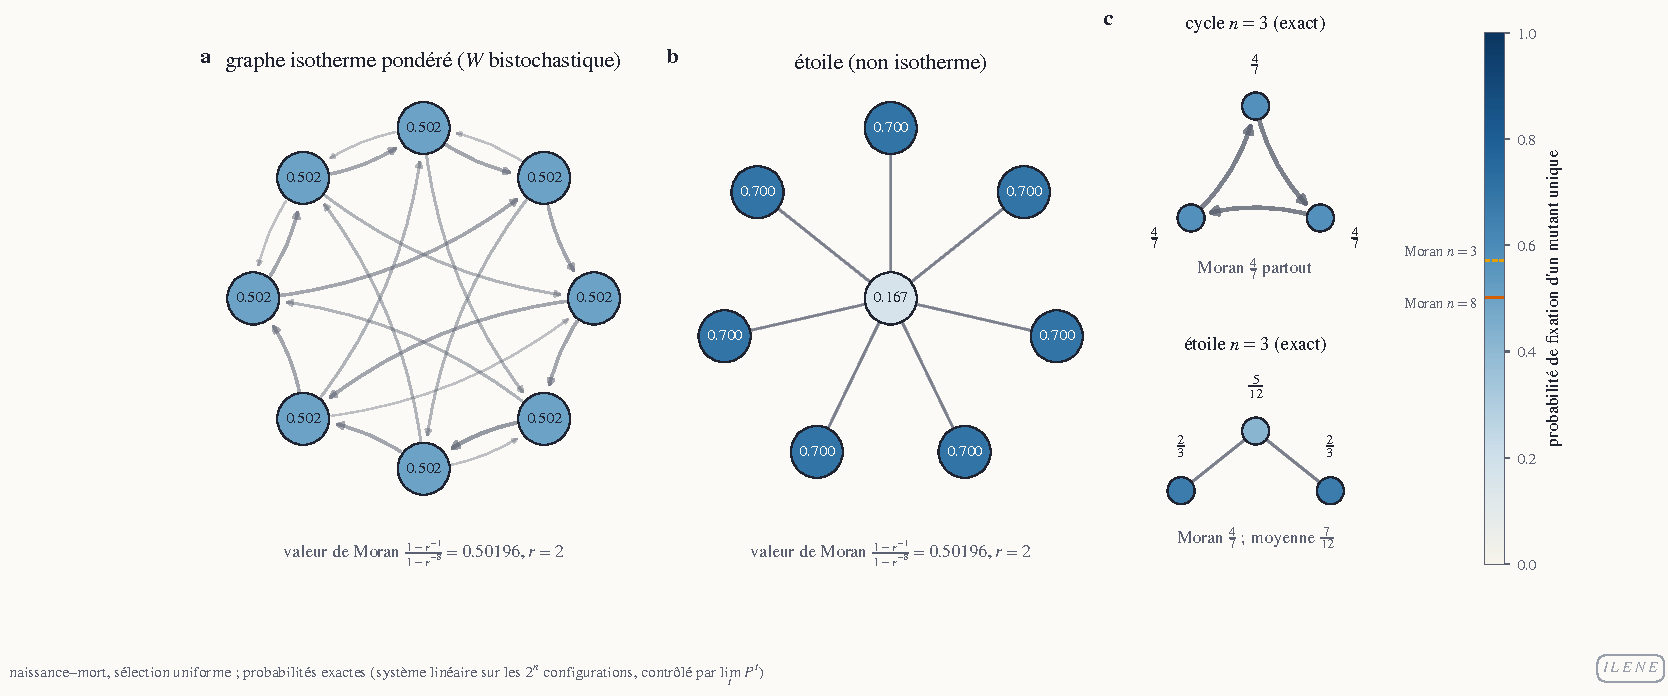
\includegraphics[width=\textwidth]{egg_ILENE.pdf}
\caption{\lean{ILENE}, \emph{Isothermal Law: Every Node Equivalent}. The theorem \tierA{}: on a strongly connected
isothermal graph ($W$ doubly stochastic), under birth--death with uniform selection, a single mutant of
fitness $r\neq1$ fixes with probability $(1-r^{-1})/(1-r^{-n})$, whatever its starting vertex. Images
\tierX{}, $r=2$, probabilities obtained by solving the linear system on the $2^n$ configurations (in floating
point for $n=8$, in rationals for $n=3$), and
checked against the limit of $P^t$. (a)~Weighted graph with $n=8$ vertices, $W=\frac12\Pi_1+\frac13\Pi_2+\frac16\Pi_3$
(three fixed-point-free permutations): all eight vertices give the Moran value $0.50196$ to within $2\cdot10^{-15}$.
(b)~The star with 7 leaves is not isothermal and lies outside the hypotheses: centre $0.167$, leaves $0.700$.
(c)~Rational computation for $n=3$: the 3-cycle gives $\frac47$ everywhere; the star gives $\frac5{12}$ at the centre and
$\frac23$ at the leaves, with mean $\frac7{12}\neq\frac47$.}
\label{fig:egg:ILENE}
\end{figure}

\begin{figure}[htbp]
\centering
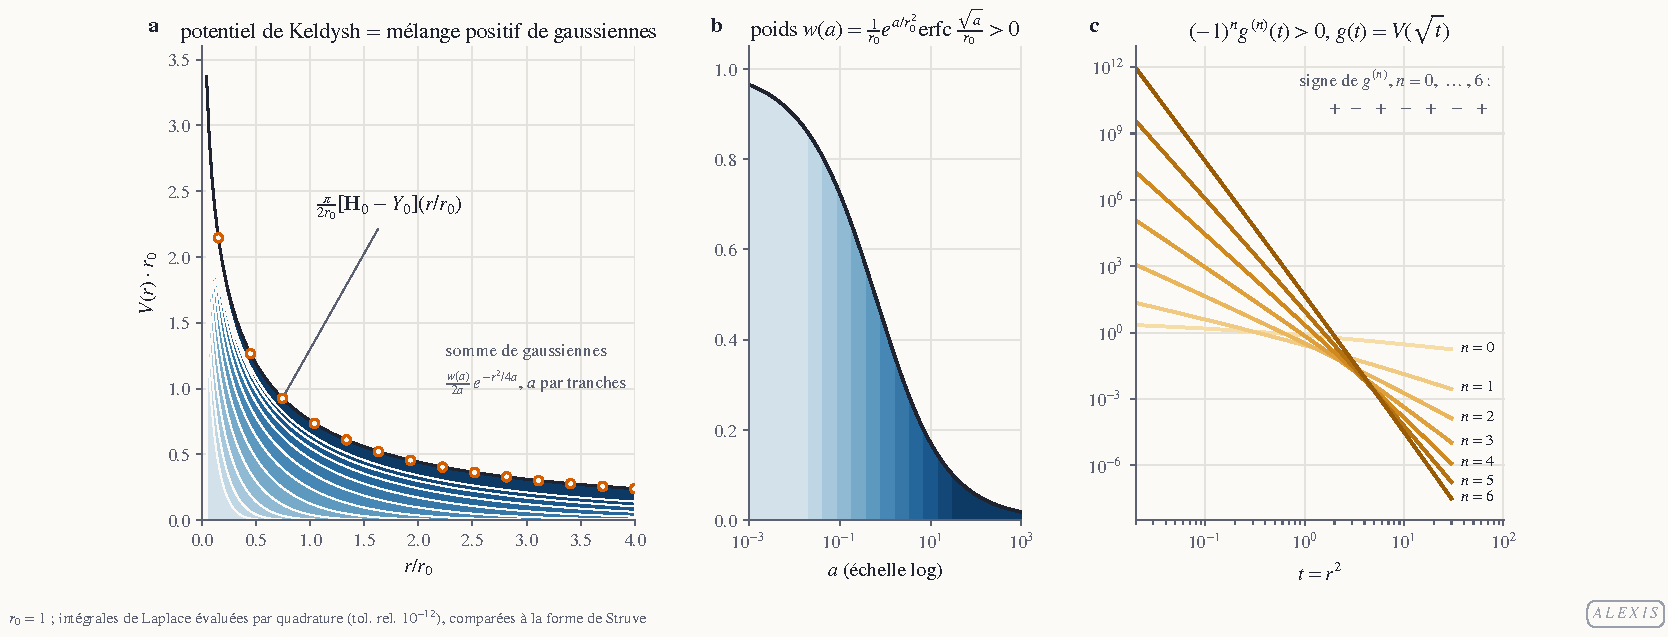
\includegraphics[width=\textwidth]{egg_ALEXIS.pdf}
\caption{\lean{ALEXIS}, \emph{Averaged Laplace EXponentials Inherit Signs}. The theorem \tierA{}: a positive
mixture of exponentials $t\mapsto\int e^{-t\,k(x)}m(x)\,d\mu(x)$ is an admissible potential, of class
$C^\infty$ on $(0,+\infty)$, positive, with $(-1)^n g^{(n)}\ge0$. The image \tierX{} shows one instance, the
Rytova--Keldysh potential ($r_0=1$), written as a Gaussian mixture
$V(r)=\int_0^\infty \frac{w(a)}{2a}\,e^{-r^2/4a}\,da$ with weight $w(a)=\frac1{r_0}e^{a/r_0^2}\operatorname{erfc}
(\sqrt a/r_0)>0$. (a)~The contributions of twelve slices in $a$, stacked, reproduce the Struve form
$\frac{\pi}{2r_0}[\mathbf H_0-Y_0](r/r_0)$ (dots) to within $3\cdot10^{-13}$ in relative terms; the identification
with the Struve form is a human proof, not machine-checked \tierC{}. (b)~The weight $w$, coloured by slice.
(c)~$(-1)^n g^{(n)}(t)$, $g(t)=V(\sqrt t)$, for $n=0,\dots,6$: all curves are positive, so the
derivatives $g^{(n)}$ alternate in sign; $n=1$ is cross-checked by finite differences of the Struve form.}
\label{fig:egg:ALEXIS}
\end{figure}

\begin{figure}[htbp]
\centering
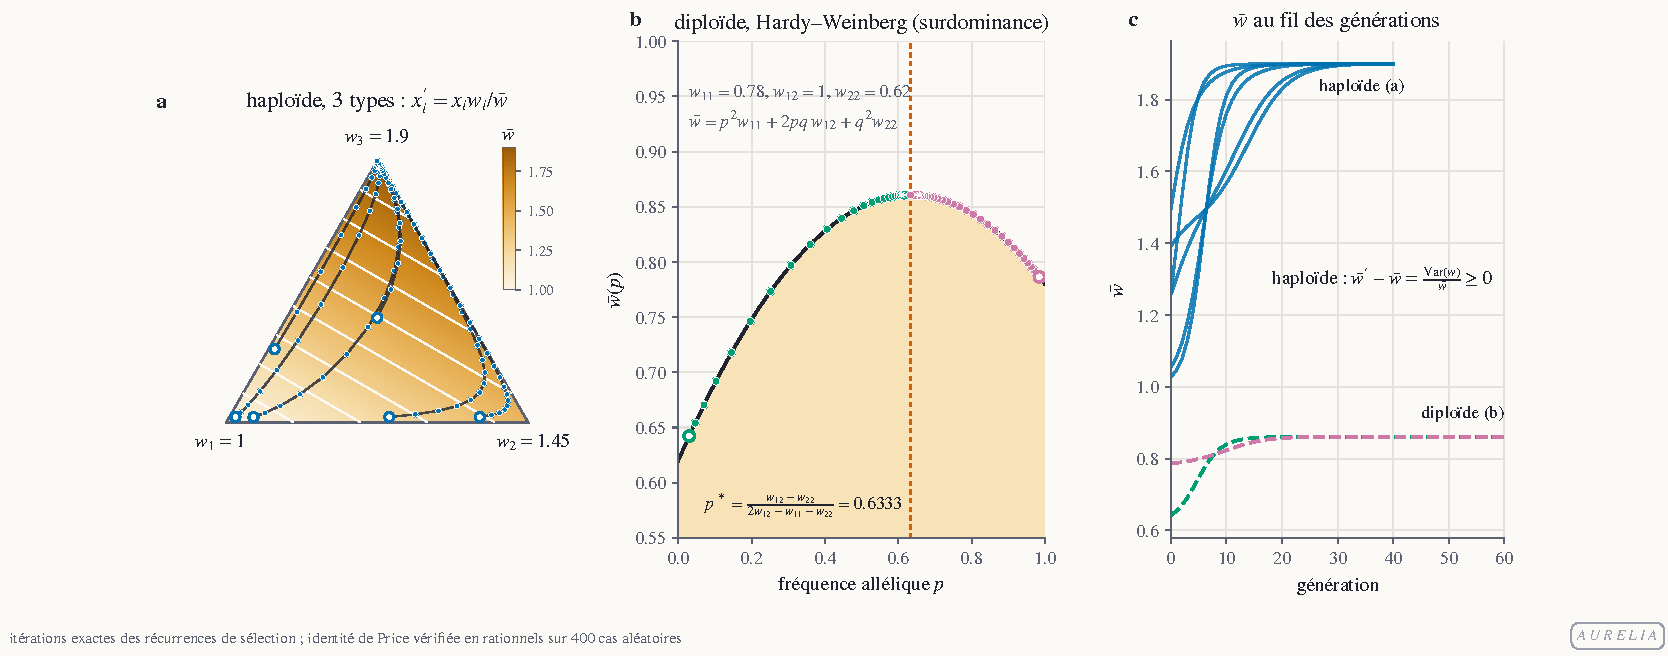
\includegraphics[width=\textwidth]{egg_AURELIA.pdf}
\caption{\lean{AURELIA}, \emph{Average Under Replication: Evolution Lifts It, Always}. The theorem \tierA{}:
under haploid selection with constant fitnesses and no transmission bias, mean fitness does not decrease,
$\bar w\le\bar w'$; this is a special case of Fisher's fundamental theorem, derived from the Price equation.
Images \tierX{}. (a)~Three types, $w=(1, 1.45, 1.9)$: on the simplex coloured by $\bar w$, six trajectories
of $x_i'=x_iw_i/\bar w$ climb towards the best type. (b)~Diploid case under Hardy--Weinberg, with overdominance
($w_{11}=0.78$, $w_{12}=1$, $w_{22}=0.62$): both trajectories climb $\bar w(p)$ up to
$p^*=0.6333$. This panel falls under the diploid theorem \lean{wbar_increment} of Chapter~4 (H12) \tierA{}, not under
\lean{AURELIA}. (c)~$\bar w$ over the generations, never decreasing. The identity
$\bar w'-\bar w=\mathrm{Var}(w)/\bar w$ is checked in exact rationals on 400 random cases; negative
control: with a mutation bias from the best type towards the worst, $\bar w$ drops by $0.35$.}
\label{fig:egg:AURELIA}
\end{figure}
).
% Figures produced by code/easter_egg_images.py (matplotlib/numpy/scipy); every plotted quantity is computed
% from its formula. The numerical self-checks (positive and negative controls) are recorded in
% results/textbook_formalisation_2026/easter_eggs_selfcheck.json; a failing check aborts the script.
\section*{The five images}
\addcontentsline{toc}{section}{The five images}

Each of the five short names of Section~\ref{ch5:acronymes} receives an image here. The tier of the theorem
(\tierA{}) refers to the re-exported Lean statement. The curves, colours and displayed values are numerical
computations \tierX{}: they illustrate a special case of the statement, without proving or extending it.

\begin{figure}[htbp]
\centering
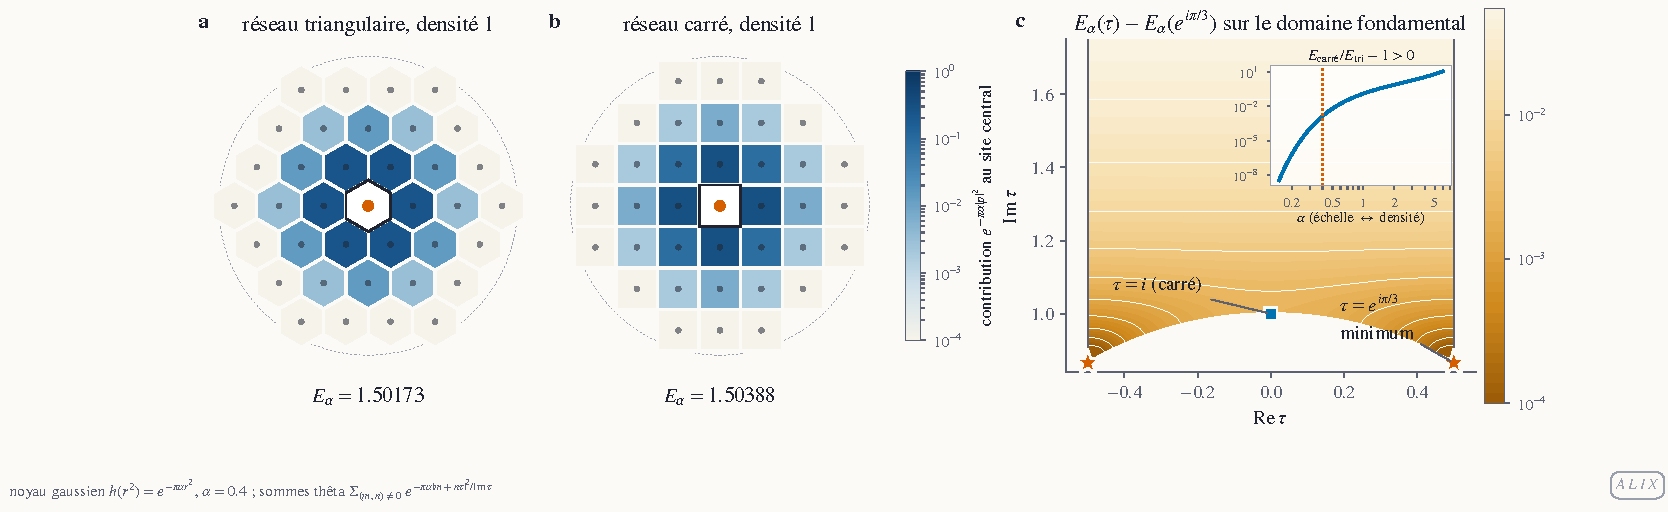
\includegraphics[width=\textwidth]{egg_ALIX.pdf}
\caption{\lean{ALIX}, \emph{A Lattice Is eXtremal}. The theorem \tierA{} (conditional on the upstream theorem
\lean{universal_energy_minimum} of openai/math, AI-generated and not peer reviewed) states that at every density
$\rho>0$ the triangular lattice minimizes the energy of every admissible potential, among all locally finite
configurations of density~$\rho$. The image \tierX{} takes the Gaussian kernel $e^{-\pi\alpha r^2}$, $\alpha=0.4$,
at density~1, and compares \emph{lattices} only. (a)~and~(b): Voronoi cells coloured by the contribution
$e^{-\pi\alpha|p|^2}$ of each site~$p$ to the energy of the central site; $E_\alpha=1.50173$ (triangular)
versus $1.50388$ (square). (c)~The difference $E_\alpha(\tau)-E_\alpha(e^{i\pi/3})$ over the fundamental domain of
lattice shapes, computed by theta sums; the grid minimum (at the equivalent point $-\tfrac12+i\tfrac{\sqrt3}2$, to within one grid step) and five
Nelder--Mead minimizations (to within $10^{-7}$) land back on $\tau=e^{i\pi/3}$. Inset: $E_{\text{square}}/E_{\text{tri}}-1>0$ for
$\alpha\in[0.15, 6]$, that is, for a whole range of densities.}
\label{fig:egg:ALIX}
\end{figure}

\begin{figure}[htbp]
\centering
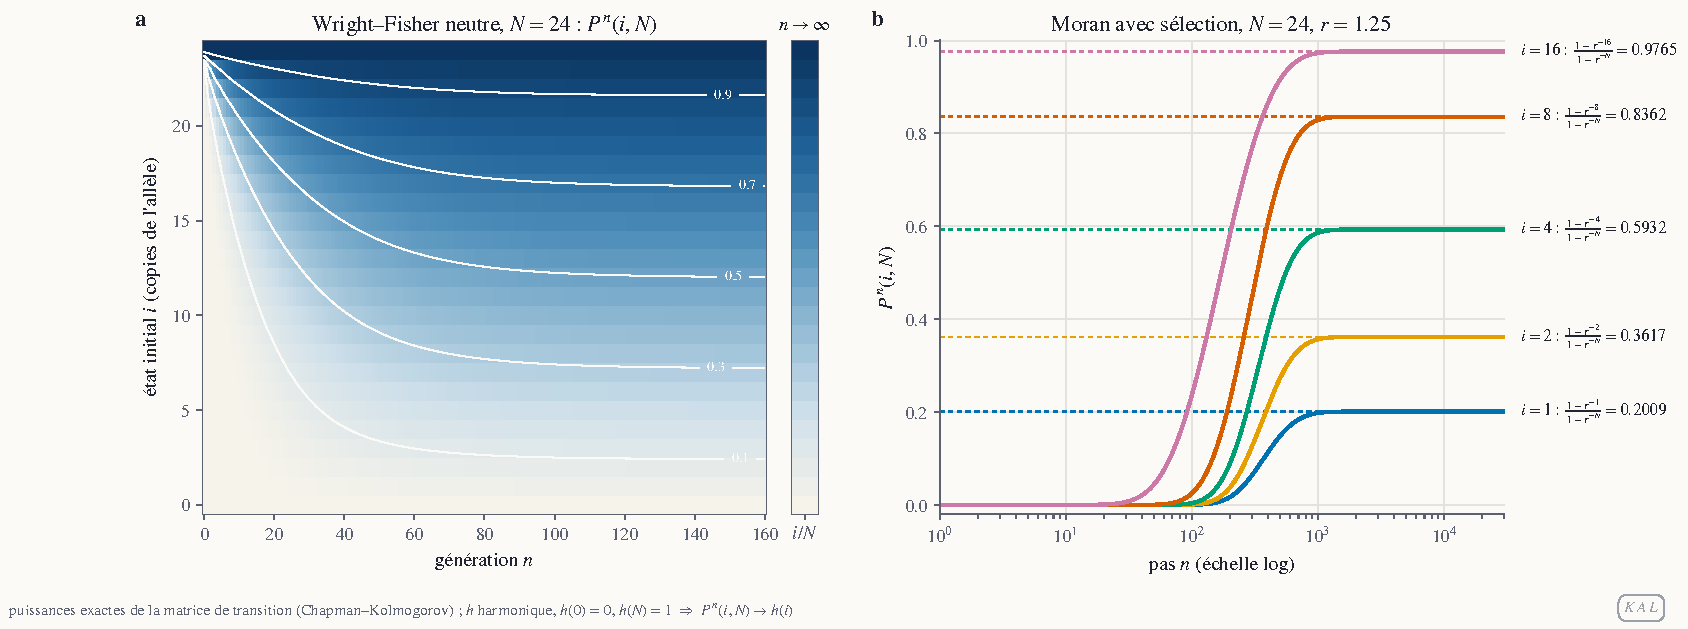
\includegraphics[width=\textwidth]{egg_KAL.pdf}
\caption{\lean{KAL}, \emph{Kolmogorov Absorption Limit}. The theorem \tierA{}: for a chain on
$\{0,\dots,N\}$ with absorbing boundaries, if $h$ is harmonic at the interior states, $h(0)=0$, $h(N)=1$, and the
one-step variance of $h$ is strictly positive, then $P^n(i,N)\to h(i)$ and $P^n(i,0)\to 1-h(i)$. Images
\tierX{}, by exact powers of the transition matrix. (a)~Neutral Wright--Fisher, $N=24$: $P^n(i,N)$
converges to $h(i)=i/N$ (right-hand band); maximal deviation at $n=4096$: $6\cdot10^{-16}$. (b)~Moran with
selection, $N=24$, $r=1.25$: $P^n(i,N)$ tends to $(1-r^{-i})/(1-r^{-N})$ (dotted), deviation
$7\cdot10^{-15}$ at $n=2^{22}$. The harmonicity of both functions $h$ is checked in exact rationals (for Wright--Fisher, at $N=8$).}
\label{fig:egg:KAL}
\end{figure}

\begin{figure}[htbp]
\centering
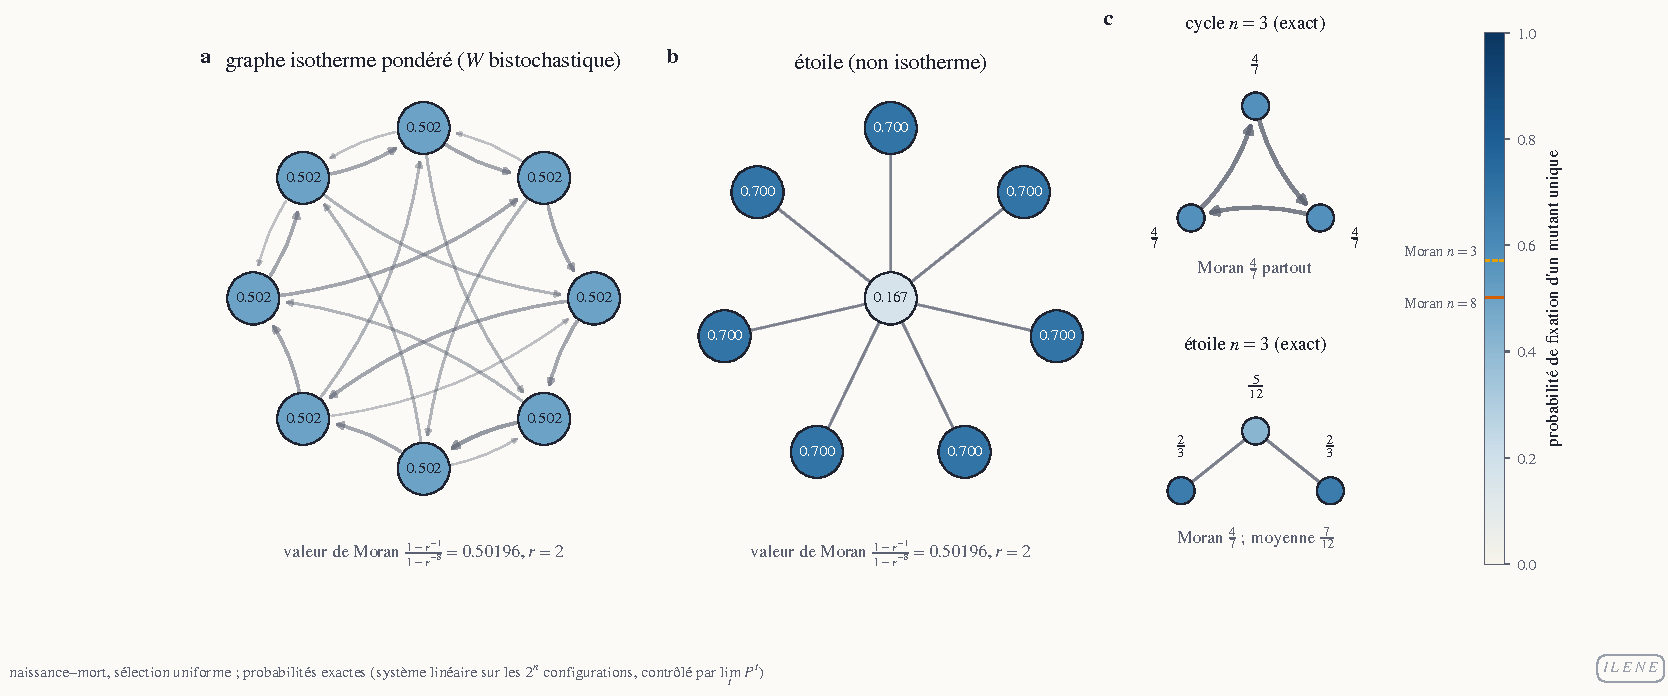
\includegraphics[width=\textwidth]{egg_ILENE.pdf}
\caption{\lean{ILENE}, \emph{Isothermal Law: Every Node Equivalent}. The theorem \tierA{}: on a strongly connected
isothermal graph ($W$ doubly stochastic), under birth--death with uniform selection, a single mutant of
fitness $r\neq1$ fixes with probability $(1-r^{-1})/(1-r^{-n})$, whatever its starting vertex. Images
\tierX{}, $r=2$, probabilities obtained by solving the linear system on the $2^n$ configurations (in floating
point for $n=8$, in rationals for $n=3$), and
checked against the limit of $P^t$. (a)~Weighted graph with $n=8$ vertices, $W=\frac12\Pi_1+\frac13\Pi_2+\frac16\Pi_3$
(three fixed-point-free permutations): all eight vertices give the Moran value $0.50196$ to within $2\cdot10^{-15}$.
(b)~The star with 7 leaves is not isothermal and lies outside the hypotheses: centre $0.167$, leaves $0.700$.
(c)~Rational computation for $n=3$: the 3-cycle gives $\frac47$ everywhere; the star gives $\frac5{12}$ at the centre and
$\frac23$ at the leaves, with mean $\frac7{12}\neq\frac47$.}
\label{fig:egg:ILENE}
\end{figure}

\begin{figure}[htbp]
\centering
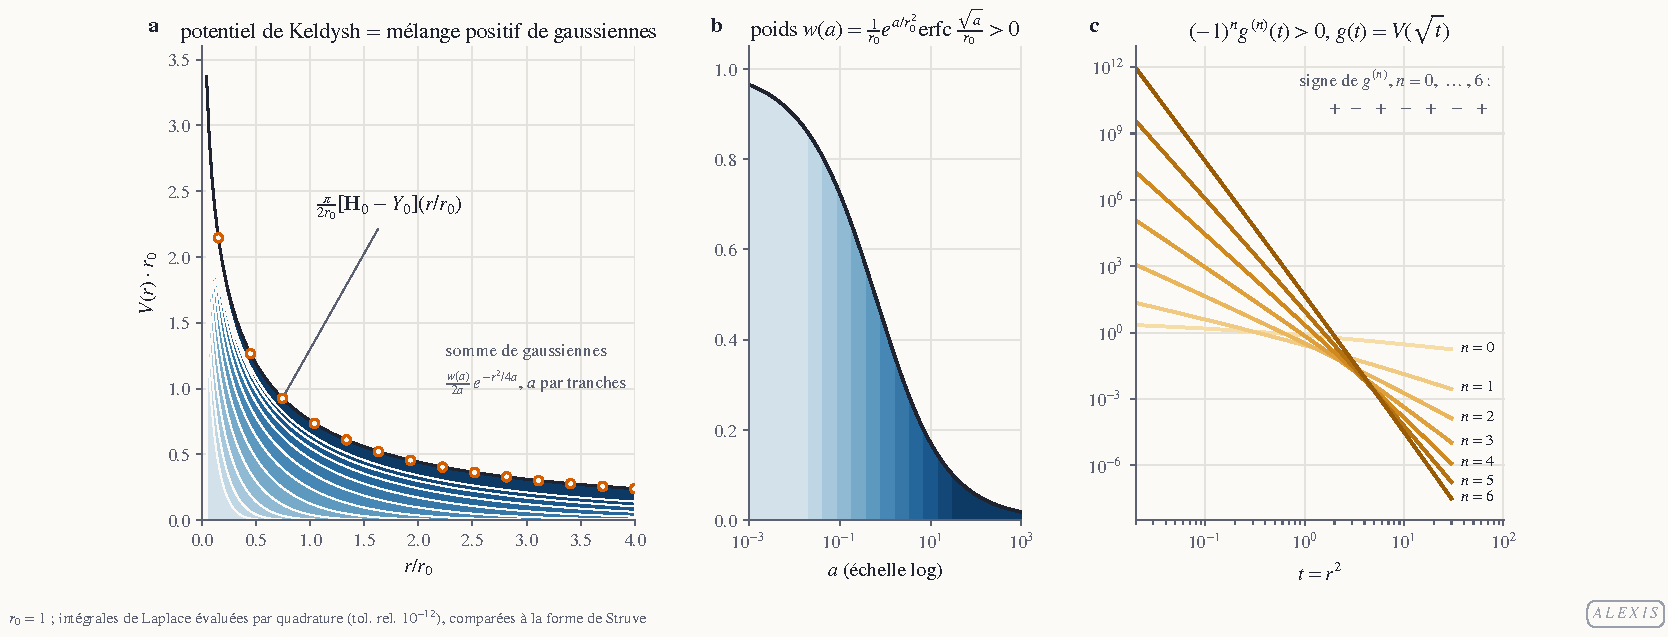
\includegraphics[width=\textwidth]{egg_ALEXIS.pdf}
\caption{\lean{ALEXIS}, \emph{Averaged Laplace EXponentials Inherit Signs}. The theorem \tierA{}: a positive
mixture of exponentials $t\mapsto\int e^{-t\,k(x)}m(x)\,d\mu(x)$ is an admissible potential, of class
$C^\infty$ on $(0,+\infty)$, positive, with $(-1)^n g^{(n)}\ge0$. The image \tierX{} shows one instance, the
Rytova--Keldysh potential ($r_0=1$), written as a Gaussian mixture
$V(r)=\int_0^\infty \frac{w(a)}{2a}\,e^{-r^2/4a}\,da$ with weight $w(a)=\frac1{r_0}e^{a/r_0^2}\operatorname{erfc}
(\sqrt a/r_0)>0$. (a)~The contributions of twelve slices in $a$, stacked, reproduce the Struve form
$\frac{\pi}{2r_0}[\mathbf H_0-Y_0](r/r_0)$ (dots) to within $3\cdot10^{-13}$ in relative terms; the identification
with the Struve form is a human proof, not machine-checked \tierC{}. (b)~The weight $w$, coloured by slice.
(c)~$(-1)^n g^{(n)}(t)$, $g(t)=V(\sqrt t)$, for $n=0,\dots,6$: all curves are positive, so the
derivatives $g^{(n)}$ alternate in sign; $n=1$ is cross-checked by finite differences of the Struve form.}
\label{fig:egg:ALEXIS}
\end{figure}

\begin{figure}[htbp]
\centering
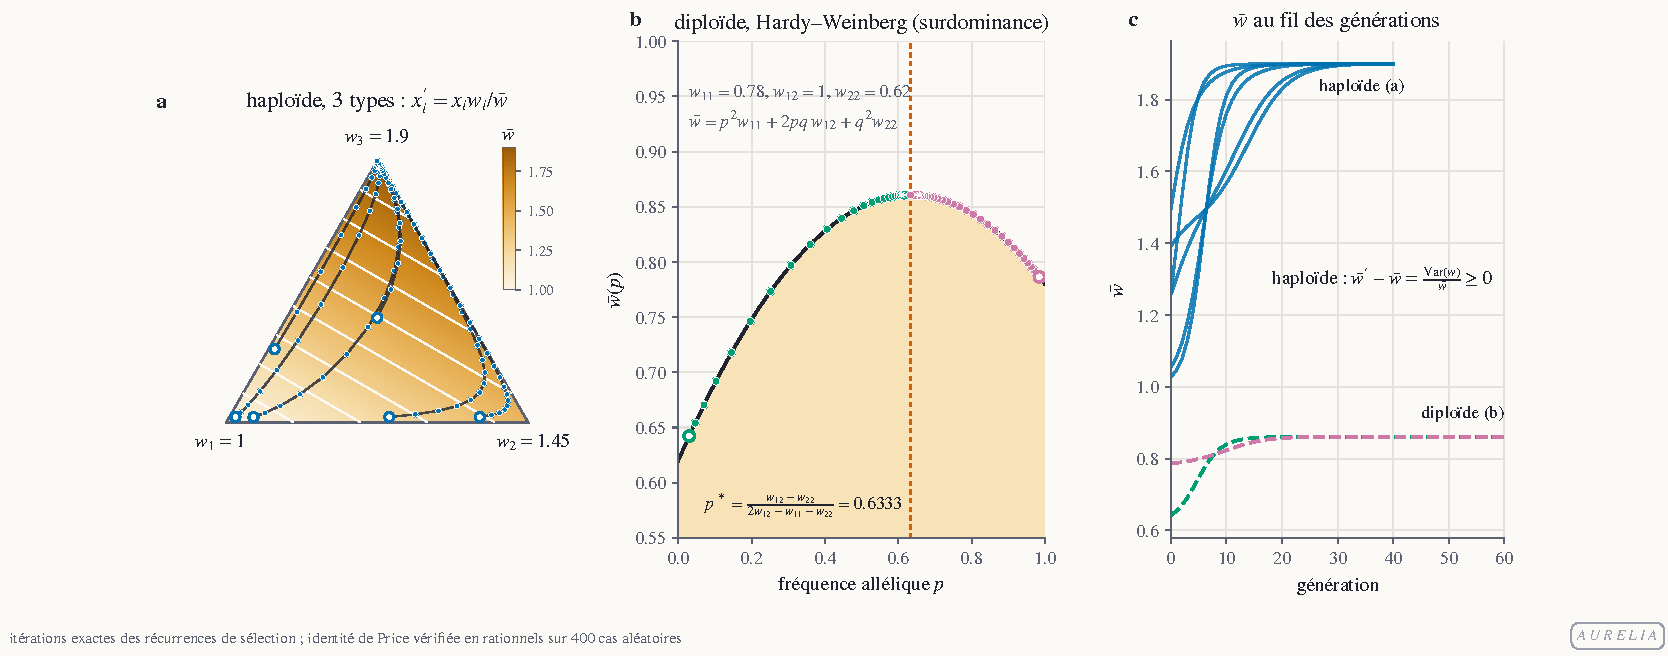
\includegraphics[width=\textwidth]{egg_AURELIA.pdf}
\caption{\lean{AURELIA}, \emph{Average Under Replication: Evolution Lifts It, Always}. The theorem \tierA{}:
under haploid selection with constant fitnesses and no transmission bias, mean fitness does not decrease,
$\bar w\le\bar w'$; this is a special case of Fisher's fundamental theorem, derived from the Price equation.
Images \tierX{}. (a)~Three types, $w=(1, 1.45, 1.9)$: on the simplex coloured by $\bar w$, six trajectories
of $x_i'=x_iw_i/\bar w$ climb towards the best type. (b)~Diploid case under Hardy--Weinberg, with overdominance
($w_{11}=0.78$, $w_{12}=1$, $w_{22}=0.62$): both trajectories climb $\bar w(p)$ up to
$p^*=0.6333$. This panel falls under the diploid theorem \lean{wbar_increment} of Chapter~4 (H12) \tierA{}, not under
\lean{AURELIA}. (c)~$\bar w$ over the generations, never decreasing. The identity
$\bar w'-\bar w=\mathrm{Var}(w)/\bar w$ is checked in exact rationals on 400 random cases; negative
control: with a mutation bias from the best type towards the worst, $\bar w$ drops by $0.35$.}
\label{fig:egg:AURELIA}
\end{figure}
).
% Figures produced by code/easter_egg_images.py (matplotlib/numpy/scipy); every plotted quantity is computed
% from its formula. The numerical self-checks (positive and negative controls) are recorded in
% results/textbook_formalisation_2026/easter_eggs_selfcheck.json; a failing check aborts the script.
\section*{The five images}
\addcontentsline{toc}{section}{The five images}

Each of the five short names of Section~\ref{ch5:acronymes} receives an image here. The tier of the theorem
(\tierA{}) refers to the re-exported Lean statement. The curves, colours and displayed values are numerical
computations \tierX{}: they illustrate a special case of the statement, without proving or extending it.

\begin{figure}[htbp]
\centering
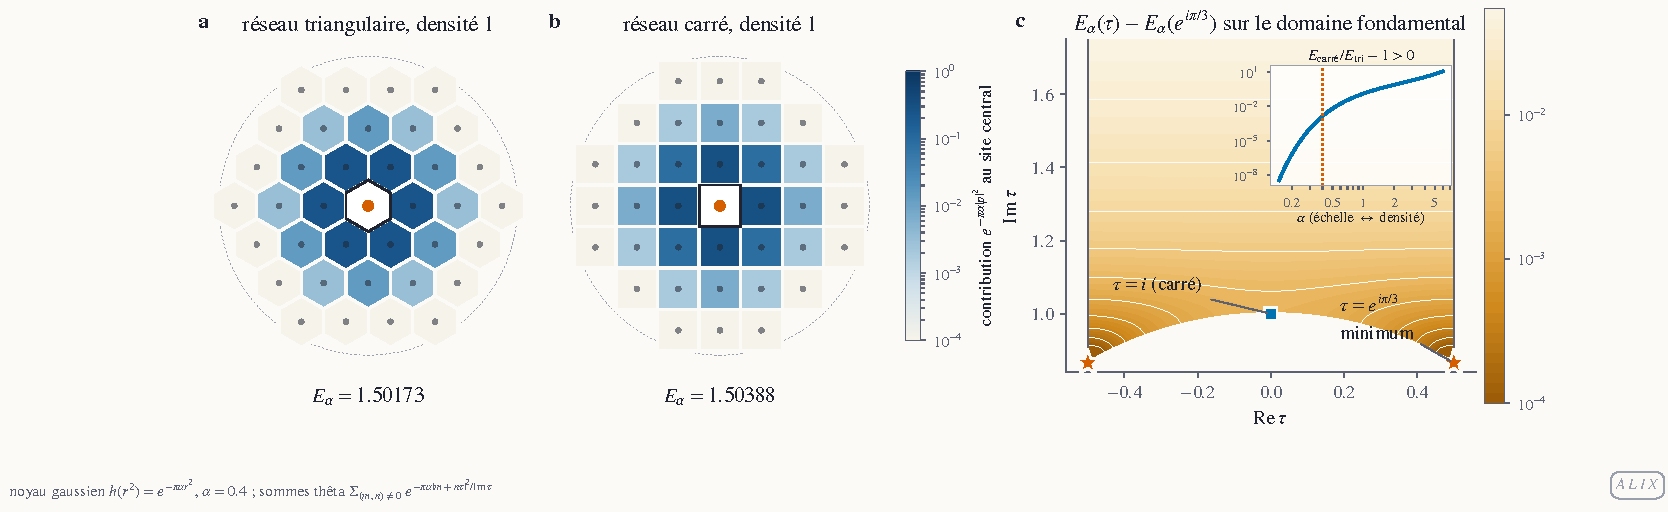
\includegraphics[width=\textwidth]{egg_ALIX.pdf}
\caption{\lean{ALIX}, \emph{A Lattice Is eXtremal}. The theorem \tierA{} (conditional on the upstream theorem
\lean{universal_energy_minimum} of openai/math, AI-generated and not peer reviewed) states that at every density
$\rho>0$ the triangular lattice minimizes the energy of every admissible potential, among all locally finite
configurations of density~$\rho$. The image \tierX{} takes the Gaussian kernel $e^{-\pi\alpha r^2}$, $\alpha=0.4$,
at density~1, and compares \emph{lattices} only. (a)~and~(b): Voronoi cells coloured by the contribution
$e^{-\pi\alpha|p|^2}$ of each site~$p$ to the energy of the central site; $E_\alpha=1.50173$ (triangular)
versus $1.50388$ (square). (c)~The difference $E_\alpha(\tau)-E_\alpha(e^{i\pi/3})$ over the fundamental domain of
lattice shapes, computed by theta sums; the grid minimum (at the equivalent point $-\tfrac12+i\tfrac{\sqrt3}2$, to within one grid step) and five
Nelder--Mead minimizations (to within $10^{-7}$) land back on $\tau=e^{i\pi/3}$. Inset: $E_{\text{square}}/E_{\text{tri}}-1>0$ for
$\alpha\in[0.15, 6]$, that is, for a whole range of densities.}
\label{fig:egg:ALIX}
\end{figure}

\begin{figure}[htbp]
\centering
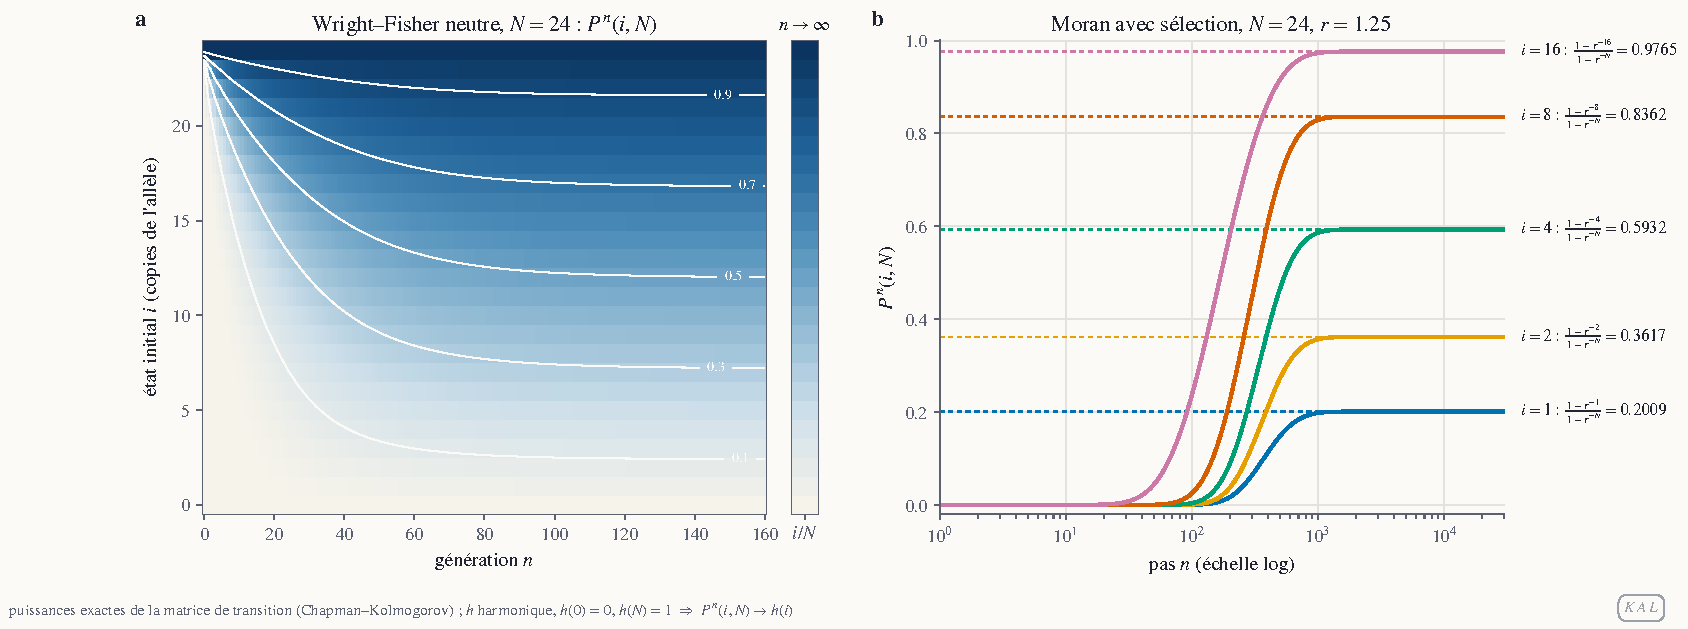
\includegraphics[width=\textwidth]{egg_KAL.pdf}
\caption{\lean{KAL}, \emph{Kolmogorov Absorption Limit}. The theorem \tierA{}: for a chain on
$\{0,\dots,N\}$ with absorbing boundaries, if $h$ is harmonic at the interior states, $h(0)=0$, $h(N)=1$, and the
one-step variance of $h$ is strictly positive, then $P^n(i,N)\to h(i)$ and $P^n(i,0)\to 1-h(i)$. Images
\tierX{}, by exact powers of the transition matrix. (a)~Neutral Wright--Fisher, $N=24$: $P^n(i,N)$
converges to $h(i)=i/N$ (right-hand band); maximal deviation at $n=4096$: $6\cdot10^{-16}$. (b)~Moran with
selection, $N=24$, $r=1.25$: $P^n(i,N)$ tends to $(1-r^{-i})/(1-r^{-N})$ (dotted), deviation
$7\cdot10^{-15}$ at $n=2^{22}$. The harmonicity of both functions $h$ is checked in exact rationals (for Wright--Fisher, at $N=8$).}
\label{fig:egg:KAL}
\end{figure}

\begin{figure}[htbp]
\centering
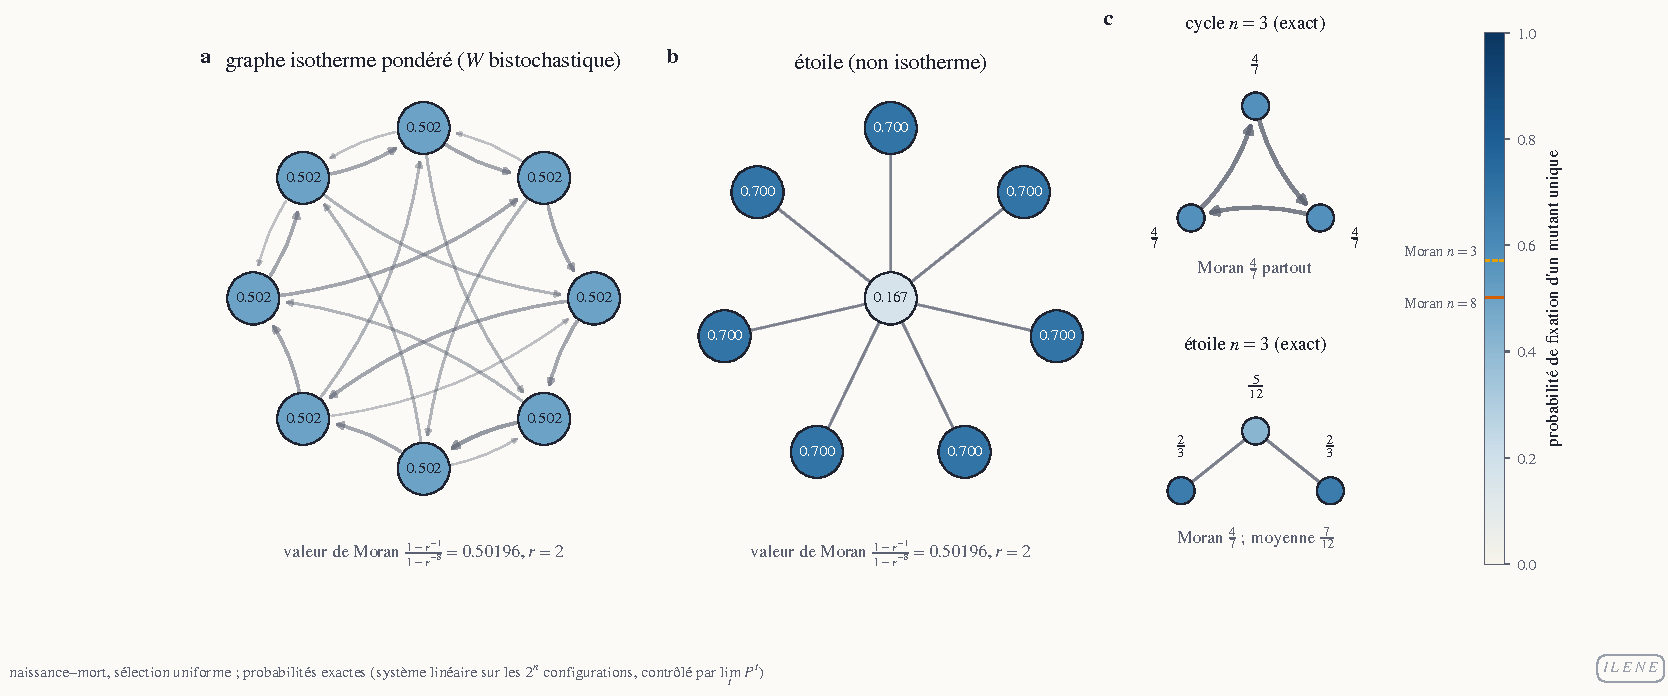
\includegraphics[width=\textwidth]{egg_ILENE.pdf}
\caption{\lean{ILENE}, \emph{Isothermal Law: Every Node Equivalent}. The theorem \tierA{}: on a strongly connected
isothermal graph ($W$ doubly stochastic), under birth--death with uniform selection, a single mutant of
fitness $r\neq1$ fixes with probability $(1-r^{-1})/(1-r^{-n})$, whatever its starting vertex. Images
\tierX{}, $r=2$, probabilities obtained by solving the linear system on the $2^n$ configurations (in floating
point for $n=8$, in rationals for $n=3$), and
checked against the limit of $P^t$. (a)~Weighted graph with $n=8$ vertices, $W=\frac12\Pi_1+\frac13\Pi_2+\frac16\Pi_3$
(three fixed-point-free permutations): all eight vertices give the Moran value $0.50196$ to within $2\cdot10^{-15}$.
(b)~The star with 7 leaves is not isothermal and lies outside the hypotheses: centre $0.167$, leaves $0.700$.
(c)~Rational computation for $n=3$: the 3-cycle gives $\frac47$ everywhere; the star gives $\frac5{12}$ at the centre and
$\frac23$ at the leaves, with mean $\frac7{12}\neq\frac47$.}
\label{fig:egg:ILENE}
\end{figure}

\begin{figure}[htbp]
\centering
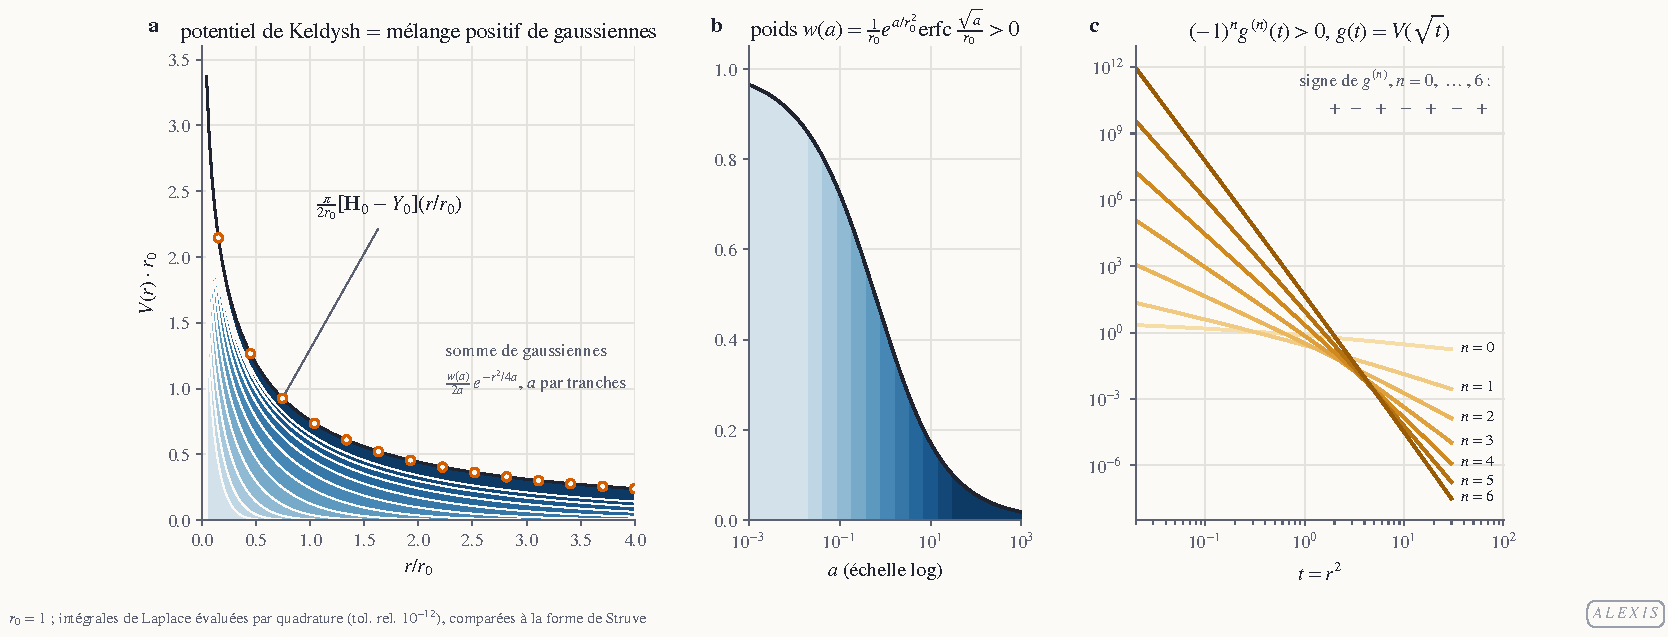
\includegraphics[width=\textwidth]{egg_ALEXIS.pdf}
\caption{\lean{ALEXIS}, \emph{Averaged Laplace EXponentials Inherit Signs}. The theorem \tierA{}: a positive
mixture of exponentials $t\mapsto\int e^{-t\,k(x)}m(x)\,d\mu(x)$ is an admissible potential, of class
$C^\infty$ on $(0,+\infty)$, positive, with $(-1)^n g^{(n)}\ge0$. The image \tierX{} shows one instance, the
Rytova--Keldysh potential ($r_0=1$), written as a Gaussian mixture
$V(r)=\int_0^\infty \frac{w(a)}{2a}\,e^{-r^2/4a}\,da$ with weight $w(a)=\frac1{r_0}e^{a/r_0^2}\operatorname{erfc}
(\sqrt a/r_0)>0$. (a)~The contributions of twelve slices in $a$, stacked, reproduce the Struve form
$\frac{\pi}{2r_0}[\mathbf H_0-Y_0](r/r_0)$ (dots) to within $3\cdot10^{-13}$ in relative terms; the identification
with the Struve form is a human proof, not machine-checked \tierC{}. (b)~The weight $w$, coloured by slice.
(c)~$(-1)^n g^{(n)}(t)$, $g(t)=V(\sqrt t)$, for $n=0,\dots,6$: all curves are positive, so the
derivatives $g^{(n)}$ alternate in sign; $n=1$ is cross-checked by finite differences of the Struve form.}
\label{fig:egg:ALEXIS}
\end{figure}

\begin{figure}[htbp]
\centering
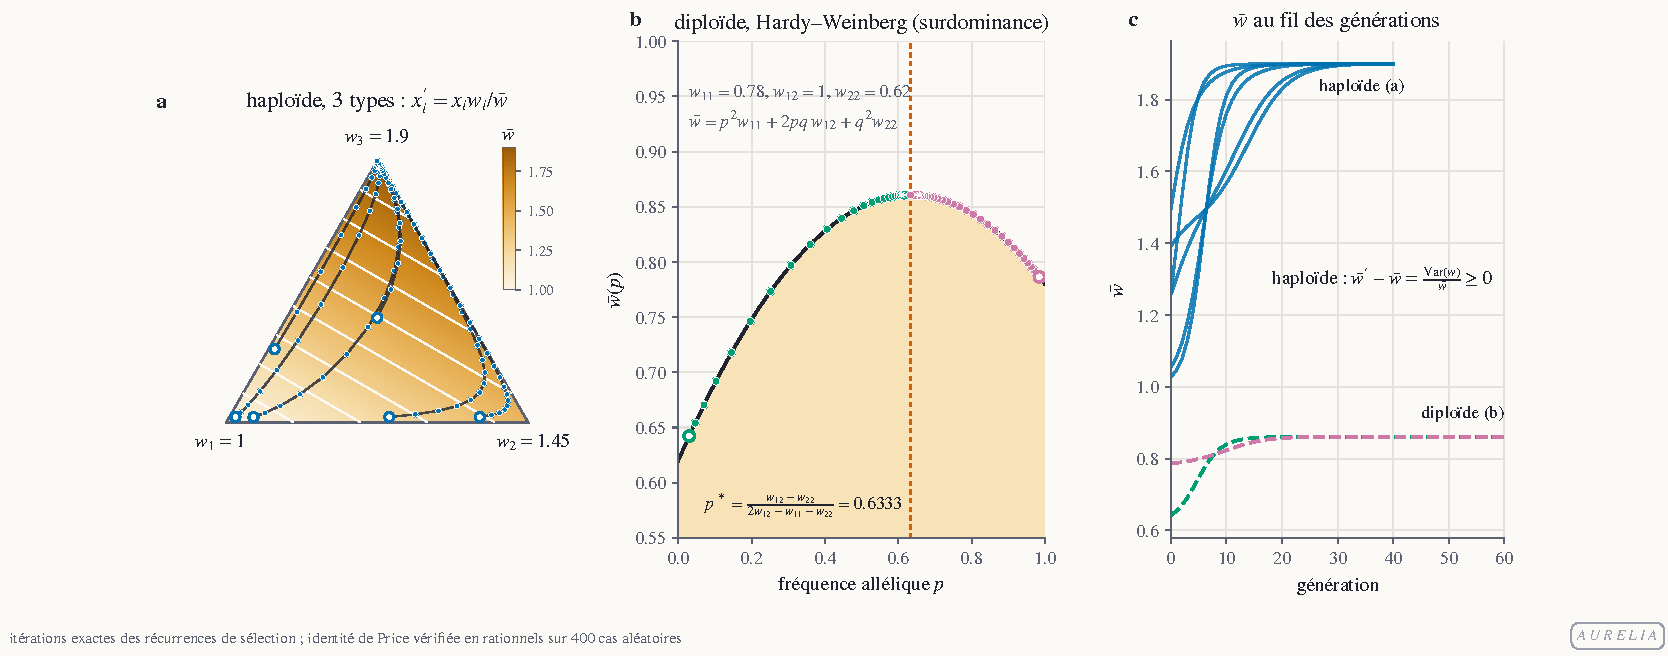
\includegraphics[width=\textwidth]{egg_AURELIA.pdf}
\caption{\lean{AURELIA}, \emph{Average Under Replication: Evolution Lifts It, Always}. The theorem \tierA{}:
under haploid selection with constant fitnesses and no transmission bias, mean fitness does not decrease,
$\bar w\le\bar w'$; this is a special case of Fisher's fundamental theorem, derived from the Price equation.
Images \tierX{}. (a)~Three types, $w=(1, 1.45, 1.9)$: on the simplex coloured by $\bar w$, six trajectories
of $x_i'=x_iw_i/\bar w$ climb towards the best type. (b)~Diploid case under Hardy--Weinberg, with overdominance
($w_{11}=0.78$, $w_{12}=1$, $w_{22}=0.62$): both trajectories climb $\bar w(p)$ up to
$p^*=0.6333$. This panel falls under the diploid theorem \lean{wbar_increment} of Chapter~4 (H12) \tierA{}, not under
\lean{AURELIA}. (c)~$\bar w$ over the generations, never decreasing. The identity
$\bar w'-\bar w=\mathrm{Var}(w)/\bar w$ is checked in exact rationals on 400 random cases; negative
control: with a mutation bias from the best type towards the worst, $\bar w$ drops by $0.35$.}
\label{fig:egg:AURELIA}
\end{figure}
).
% Figures produced by code/easter_egg_images.py (matplotlib/numpy/scipy); every plotted quantity is computed
% from its formula. The numerical self-checks (positive and negative controls) are recorded in
% results/textbook_formalisation_2026/easter_eggs_selfcheck.json; a failing check aborts the script.
\section*{The five images}
\addcontentsline{toc}{section}{The five images}

Each of the five short names of Section~\ref{ch5:acronymes} receives an image here. The tier of the theorem
(\tierA{}) refers to the re-exported Lean statement. The curves, colours and displayed values are numerical
computations \tierX{}: they illustrate a special case of the statement, without proving or extending it.

\begin{figure}[htbp]
\centering
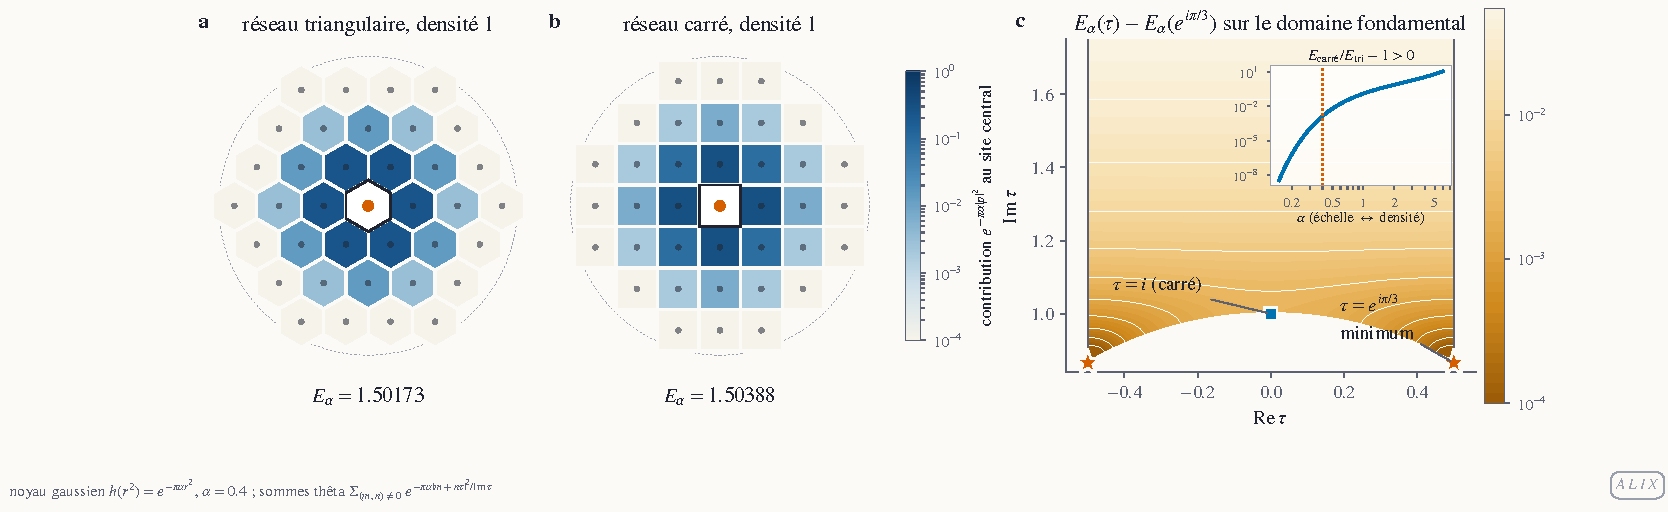
\includegraphics[width=\textwidth]{egg_ALIX.pdf}
\caption{\lean{ALIX}, \emph{A Lattice Is eXtremal}. The theorem \tierA{} (conditional on the upstream theorem
\lean{universal_energy_minimum} of openai/math, AI-generated and not peer reviewed) states that at every density
$\rho>0$ the triangular lattice minimizes the energy of every admissible potential, among all locally finite
configurations of density~$\rho$. The image \tierX{} takes the Gaussian kernel $e^{-\pi\alpha r^2}$, $\alpha=0.4$,
at density~1, and compares \emph{lattices} only. (a)~and~(b): Voronoi cells coloured by the contribution
$e^{-\pi\alpha|p|^2}$ of each site~$p$ to the energy of the central site; $E_\alpha=1.50173$ (triangular)
versus $1.50388$ (square). (c)~The difference $E_\alpha(\tau)-E_\alpha(e^{i\pi/3})$ over the fundamental domain of
lattice shapes, computed by theta sums; the grid minimum (at the equivalent point $-\tfrac12+i\tfrac{\sqrt3}2$, to within one grid step) and five
Nelder--Mead minimizations (to within $10^{-7}$) land back on $\tau=e^{i\pi/3}$. Inset: $E_{\text{square}}/E_{\text{tri}}-1>0$ for
$\alpha\in[0.15, 6]$, that is, for a whole range of densities.}
\label{fig:egg:ALIX}
\end{figure}

\begin{figure}[htbp]
\centering
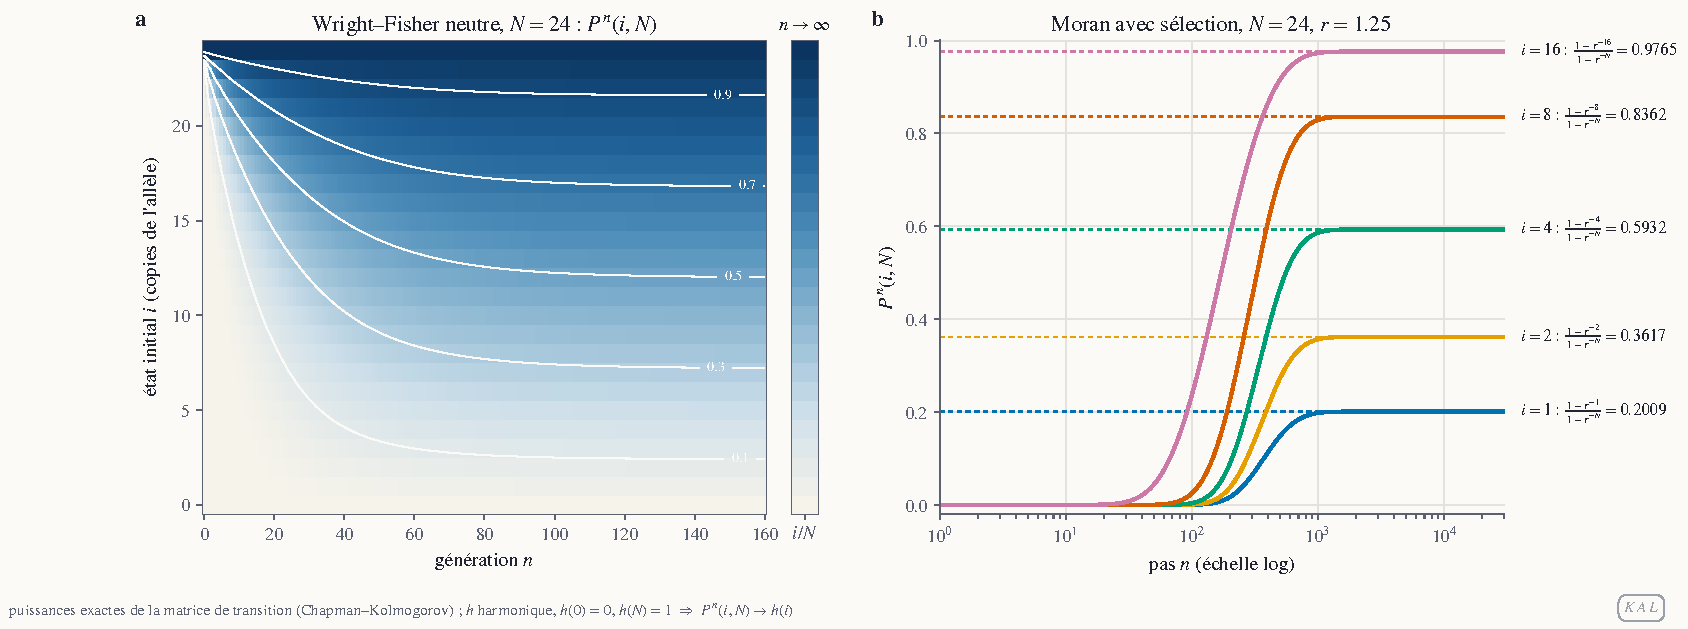
\includegraphics[width=\textwidth]{egg_KAL.pdf}
\caption{\lean{KAL}, \emph{Kolmogorov Absorption Limit}. The theorem \tierA{}: for a chain on
$\{0,\dots,N\}$ with absorbing boundaries, if $h$ is harmonic at the interior states, $h(0)=0$, $h(N)=1$, and the
one-step variance of $h$ is strictly positive, then $P^n(i,N)\to h(i)$ and $P^n(i,0)\to 1-h(i)$. Images
\tierX{}, by exact powers of the transition matrix. (a)~Neutral Wright--Fisher, $N=24$: $P^n(i,N)$
converges to $h(i)=i/N$ (right-hand band); maximal deviation at $n=4096$: $6\cdot10^{-16}$. (b)~Moran with
selection, $N=24$, $r=1.25$: $P^n(i,N)$ tends to $(1-r^{-i})/(1-r^{-N})$ (dotted), deviation
$7\cdot10^{-15}$ at $n=2^{22}$. The harmonicity of both functions $h$ is checked in exact rationals (for Wright--Fisher, at $N=8$).}
\label{fig:egg:KAL}
\end{figure}

\begin{figure}[htbp]
\centering
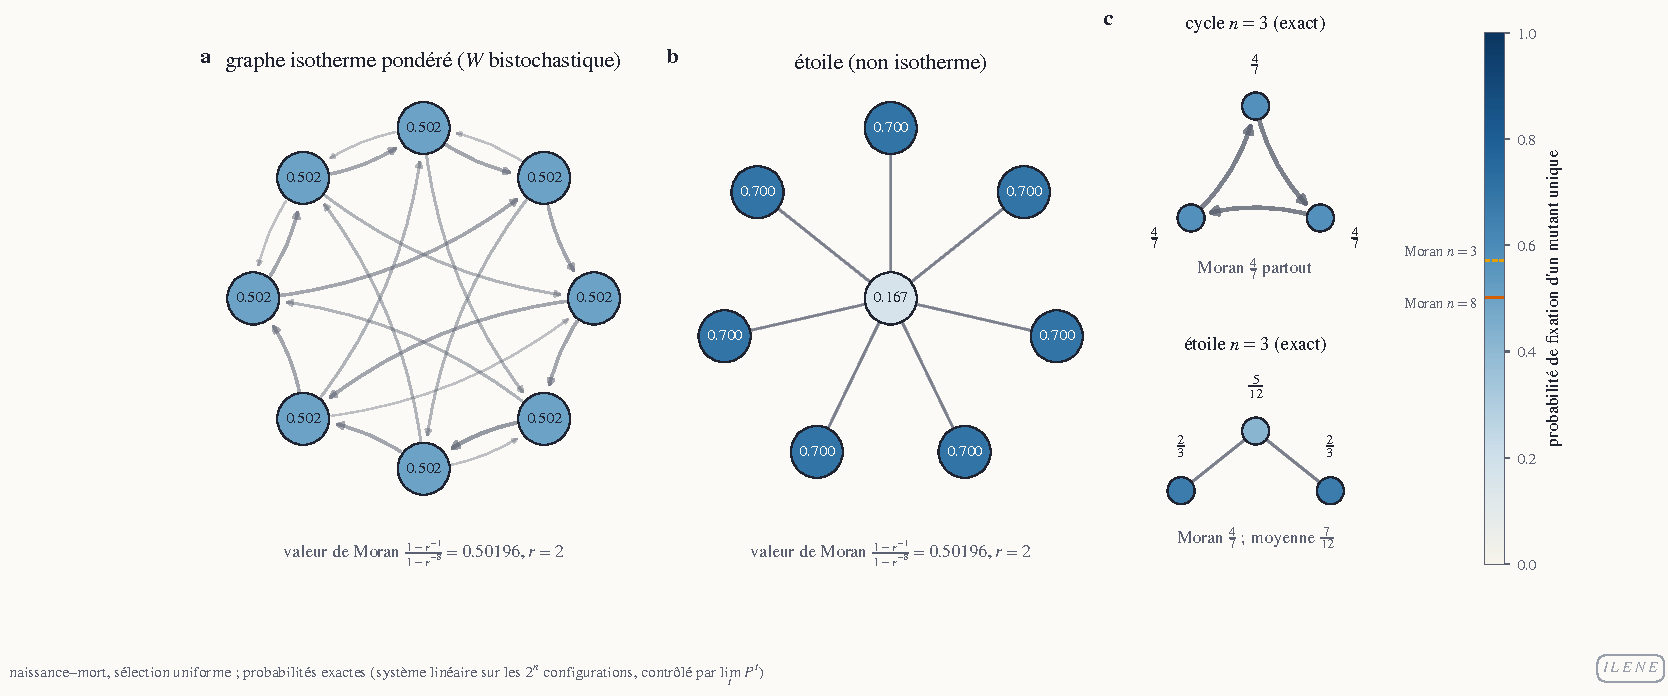
\includegraphics[width=\textwidth]{egg_ILENE.pdf}
\caption{\lean{ILENE}, \emph{Isothermal Law: Every Node Equivalent}. The theorem \tierA{}: on a strongly connected
isothermal graph ($W$ doubly stochastic), under birth--death with uniform selection, a single mutant of
fitness $r\neq1$ fixes with probability $(1-r^{-1})/(1-r^{-n})$, whatever its starting vertex. Images
\tierX{}, $r=2$, probabilities obtained by solving the linear system on the $2^n$ configurations (in floating
point for $n=8$, in rationals for $n=3$), and
checked against the limit of $P^t$. (a)~Weighted graph with $n=8$ vertices, $W=\frac12\Pi_1+\frac13\Pi_2+\frac16\Pi_3$
(three fixed-point-free permutations): all eight vertices give the Moran value $0.50196$ to within $2\cdot10^{-15}$.
(b)~The star with 7 leaves is not isothermal and lies outside the hypotheses: centre $0.167$, leaves $0.700$.
(c)~Rational computation for $n=3$: the 3-cycle gives $\frac47$ everywhere; the star gives $\frac5{12}$ at the centre and
$\frac23$ at the leaves, with mean $\frac7{12}\neq\frac47$.}
\label{fig:egg:ILENE}
\end{figure}

\begin{figure}[htbp]
\centering
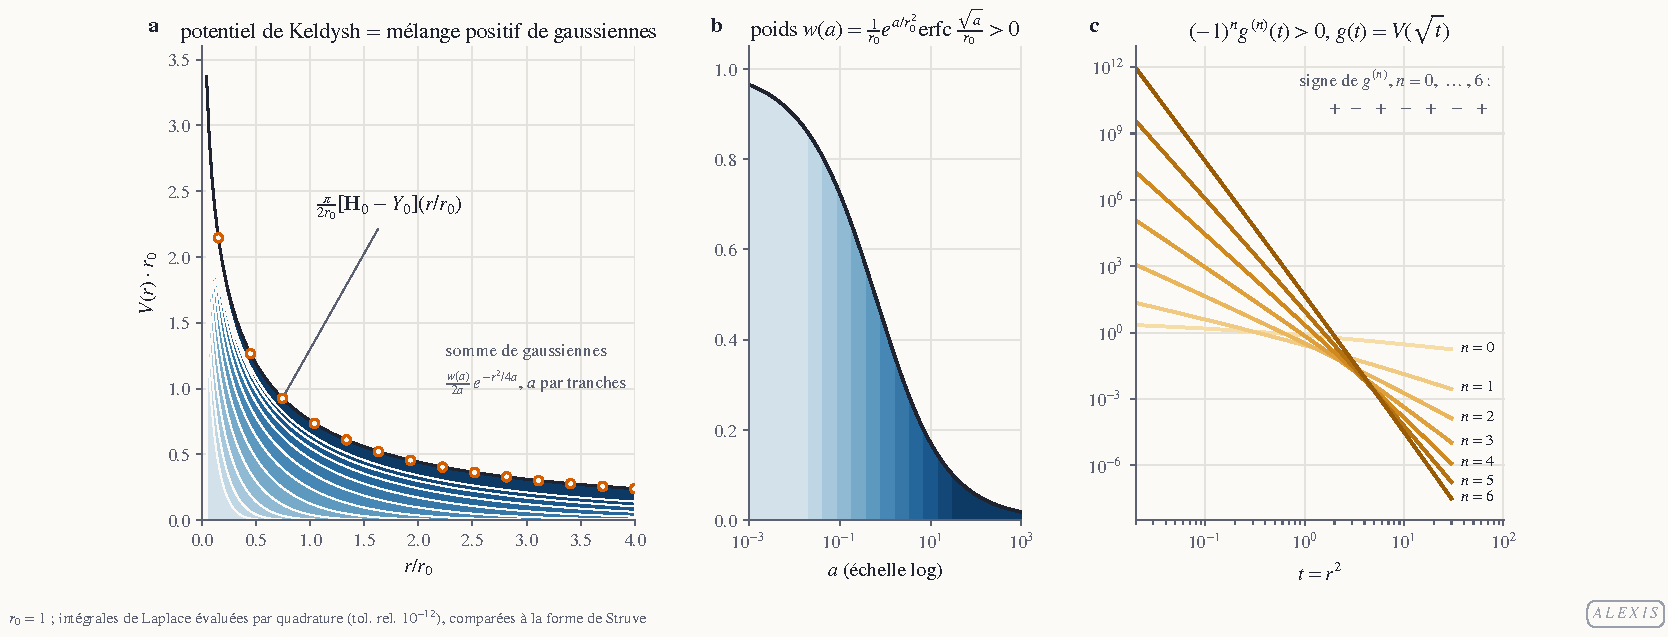
\includegraphics[width=\textwidth]{egg_ALEXIS.pdf}
\caption{\lean{ALEXIS}, \emph{Averaged Laplace EXponentials Inherit Signs}. The theorem \tierA{}: a positive
mixture of exponentials $t\mapsto\int e^{-t\,k(x)}m(x)\,d\mu(x)$ is an admissible potential, of class
$C^\infty$ on $(0,+\infty)$, positive, with $(-1)^n g^{(n)}\ge0$. The image \tierX{} shows one instance, the
Rytova--Keldysh potential ($r_0=1$), written as a Gaussian mixture
$V(r)=\int_0^\infty \frac{w(a)}{2a}\,e^{-r^2/4a}\,da$ with weight $w(a)=\frac1{r_0}e^{a/r_0^2}\operatorname{erfc}
(\sqrt a/r_0)>0$. (a)~The contributions of twelve slices in $a$, stacked, reproduce the Struve form
$\frac{\pi}{2r_0}[\mathbf H_0-Y_0](r/r_0)$ (dots) to within $3\cdot10^{-13}$ in relative terms; the identification
with the Struve form is a human proof, not machine-checked \tierC{}. (b)~The weight $w$, coloured by slice.
(c)~$(-1)^n g^{(n)}(t)$, $g(t)=V(\sqrt t)$, for $n=0,\dots,6$: all curves are positive, so the
derivatives $g^{(n)}$ alternate in sign; $n=1$ is cross-checked by finite differences of the Struve form.}
\label{fig:egg:ALEXIS}
\end{figure}

\begin{figure}[htbp]
\centering
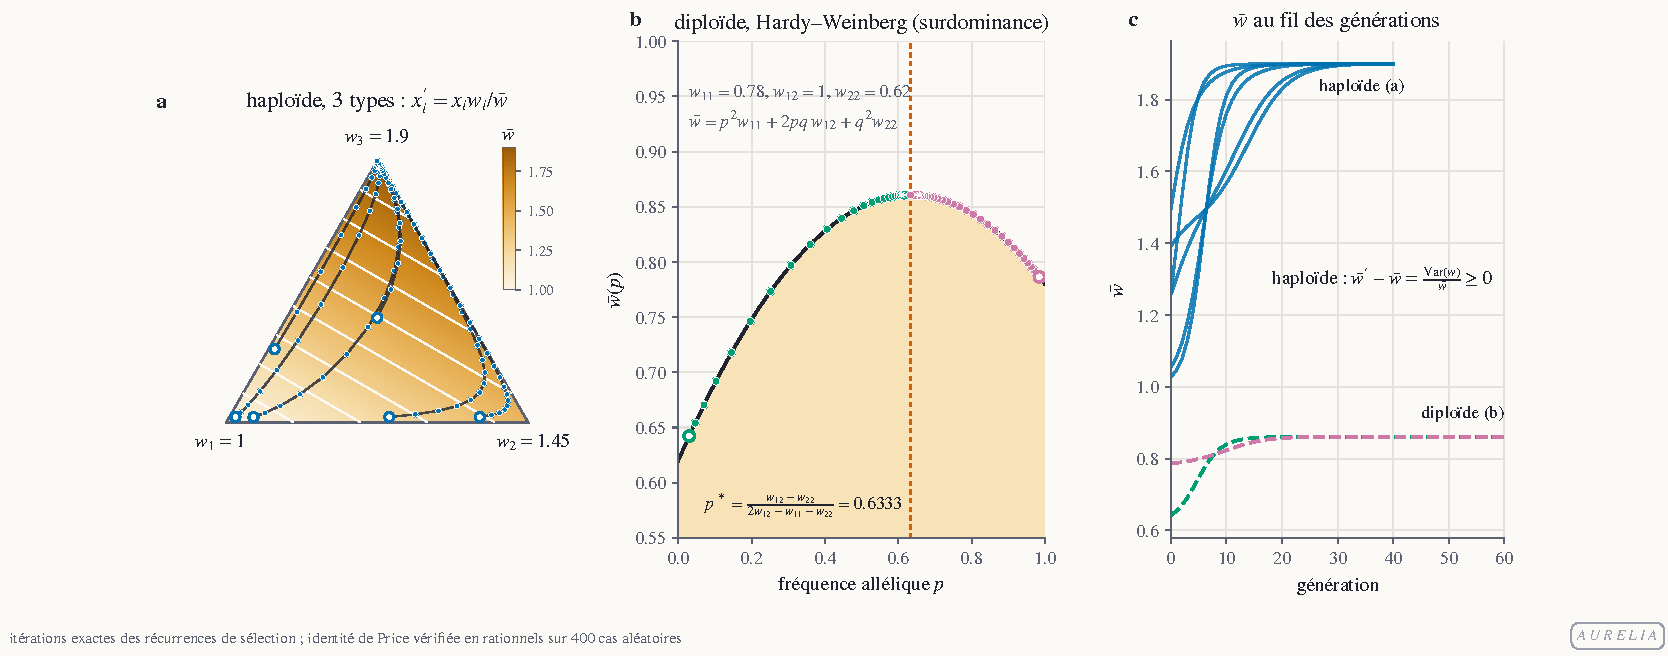
\includegraphics[width=\textwidth]{egg_AURELIA.pdf}
\caption{\lean{AURELIA}, \emph{Average Under Replication: Evolution Lifts It, Always}. The theorem \tierA{}:
under haploid selection with constant fitnesses and no transmission bias, mean fitness does not decrease,
$\bar w\le\bar w'$; this is a special case of Fisher's fundamental theorem, derived from the Price equation.
Images \tierX{}. (a)~Three types, $w=(1, 1.45, 1.9)$: on the simplex coloured by $\bar w$, six trajectories
of $x_i'=x_iw_i/\bar w$ climb towards the best type. (b)~Diploid case under Hardy--Weinberg, with overdominance
($w_{11}=0.78$, $w_{12}=1$, $w_{22}=0.62$): both trajectories climb $\bar w(p)$ up to
$p^*=0.6333$. This panel falls under the diploid theorem \lean{wbar_increment} of Chapter~4 (H12) \tierA{}, not under
\lean{AURELIA}. (c)~$\bar w$ over the generations, never decreasing. The identity
$\bar w'-\bar w=\mathrm{Var}(w)/\bar w$ is checked in exact rationals on 400 random cases; negative
control: with a mutation bias from the best type towards the worst, $\bar w$ drops by $0.35$.}
\label{fig:egg:AURELIA}
\end{figure}
